
\documentclass{article}


\usepackage{lmodern}
\usepackage[german]{babel} 
\usepackage{csquotes}
\MakeOuterQuote{"} 

\usepackage{graphicx}
\usepackage{enumerate}

\usepackage{amssymb}
\usepackage{amsmath}
\usepackage{amsthm}
\usepackage{dsfont}
\usepackage{bm}

\usepackage{caption}
\usepackage{subcaption}
\usepackage{tikz}
\usetikzlibrary{cd}

\usepackage{hyperref}
\hypersetup{
	colorlinks  = true,
	urlcolor    = LMUpurple,
	linkcolor   = LMUgreen,
	citecolor   = LMUgreen
}
\usepackage[capitalize,nameinlink]{cleveref}
\Crefname{chapter}{Kapitel}{Kapitel}
\Crefname{section}{Abschnitt}{Abschnitte}
\Crefname{subsection}{Abschnitt}{Abschnitte}
\Crefname{figure}{Abbildung}{Abbildungen}
\Crefname{subfigure}{Abbildung}{Abbildungen}

\usepackage{bookmark}

\usepackage[landscape]{geometry}
\usepackage{url}
\usepackage{multicol}
\usepackage{esint}
\usetikzlibrary{decorations.pathmorphing}
\usepackage{colortbl}
\usepackage{xcolor}
\usepackage{mathtools}
\usepackage{listings}

\lstset{language=R,
    basicstyle=\small\ttfamily,
    stringstyle=\color{purple},
    otherkeywords={0,1,2,3,4,5,6,7,8,9},
    morekeywords={TRUE,FALSE},
    deletekeywords={data,frame,length,as,character},
    keywordstyle=\color{blue},
    commentstyle=\color{purple},
}


%\usepackage{blindtext}
\usepackage{subfiles}
\makeatletter


\usepackage{bm}
\usepackage{dsfont}

% blackboard bold 
\newcommand{\ind}{\mathds{1}}
\newcommand{\R}{\mathds{R}}
\newcommand{\N}{\mathds{N}}
\newcommand{\Q}{\mathds{Q}}
\providecommand{\C}{}
\renewcommand{\C}{\mathds{C}}
\providecommand{\P}{}
\renewcommand{\P}{\mathds{P}}
\newcommand{\Z}{\mathds{Z}}
\newcommand{\E}{\mathds{E}}
\newcommand{\K}{\mathds{K}}
\renewcommand{\L}{\mathds{L}}
\newcommand{\F}{\mathds{F}}
\providecommand{\G}{}
\newcommand{\D}{\mathds{D}}

% bold letters
\newcommand{\bnull}{\bm{0}}
\newcommand{\ba}{\bm{a}}
\newcommand{\bb}{\bm{b}}
\newcommand{\bc}{\bm{c}}
\newcommand{\bd}{\bm{d}}
\newcommand{\be}{\bm{e}}
% \newcommand{\bf}{\bm{f}}
\newcommand{\bg}{\bm{g}}
\newcommand{\bh}{\bm{h}}
\newcommand{\bi}{\bm{i}}
\newcommand{\bj}{\bm{j}}
\newcommand{\bk}{\bm{k}}
\newcommand{\bl}{\bm{l}}
% \newcommand{\bm}{\bm{m}}
\newcommand{\bn}{\bm{n}}
\newcommand{\bo}{\bm{o}}
\newcommand{\bp}{\bm{p}}
\newcommand{\bq}{\bm{q}}
\newcommand{\br}{\bm{r}}
\newcommand{\bs}{\bm{s}}
\newcommand{\bt}{\bm{t}}
\newcommand{\bu}{\bm{u}}
\newcommand{\bv}{\bm{v}}
\newcommand{\bw}{\bm{w}}
\newcommand{\bx}{\bm{x}}
\newcommand{\by}{\bm{y}}
\newcommand{\bz}{\bm{z}}

% bold letters
\newcommand{\bA}{\bm{A}}
\newcommand{\bB}{\bm{B}}
\newcommand{\bC}{\bm{C}}
\newcommand{\bD}{\bm{D}}
\newcommand{\bE}{\bm{E}}
% \newcommand{\bf}{\bm{f}}
\newcommand{\bG}{\bm{G}}
\newcommand{\bH}{\bm{H}}
\newcommand{\bI}{\bm{I}}
\newcommand{\bJ}{\bm{J}}
\newcommand{\bK}{\bm{K}}
\newcommand{\bL}{\bm{L}}
\newcommand{\bM}{\bm{M}}
\newcommand{\bN}{\bm{N}}
\newcommand{\bO}{\bm{O}}
\newcommand{\bP}{\bm{P}}
\newcommand{\bQ}{\bm{Q}}
\newcommand{\bR}{\bm{R}}
\newcommand{\bS}{\bm{S}}
\newcommand{\bT}{\bm{T}}
\newcommand{\bU}{\bm{U}}
\newcommand{\bV}{\bm{V}}
\newcommand{\bW}{\bm{W}}
\newcommand{\bX}{\bm{X}}
\newcommand{\bY}{\bm{Y}}
\newcommand{\bZ}{\bm{Z}}


% calligraphic letters
\newcommand{\Acal}{\mathcal{A}}
\newcommand{\Bcal}{\mathcal{B}}
\newcommand{\Ccal}{\mathcal{C}}
\newcommand{\Dcal}{\mathcal{D}}
\newcommand{\Ecal}{\mathcal{E}}
\newcommand{\Fcal}{\mathcal{F}}
\newcommand{\Gcal}{\mathcal{G}}
\newcommand{\Hcal}{\mathcal{H}}
\newcommand{\Ical}{\mathcal{I}}
\newcommand{\Jcal}{\mathcal{J}}
\newcommand{\Kcal}{\mathcal{K}}
\newcommand{\Lcal}{\mathcal{L}}
\newcommand{\Mcal}{\mathcal{M}}
\newcommand{\Ncal}{\mathcal{N}}
\newcommand{\Ocal}{\mathcal{O}}
\newcommand{\Pcal}{\mathcal{P}}
\newcommand{\Qcal}{\mathcal{Q}}
\newcommand{\Rcal}{\mathcal{R}}
\newcommand{\Scal}{\mathcal{S}}
\newcommand{\Tcal}{\mathcal{T}}
\newcommand{\Ucal}{\mathcal{U}}
\newcommand{\Vcal}{\mathcal{V}}
\newcommand{\Wcal}{\mathcal{W}}
\newcommand{\Xcal}{\mathcal{X}}
\newcommand{\Ycal}{\mathcal{Y}}
\newcommand{\Zcal}{\mathcal{Z}}

% greek letters
\newcommand{\eps}{\varepsilon}
\newcommand{\sd}{\sigma}
\newcommand{\ssd}{\sigma^2}
\newcommand{\hbe}{\hat{\beta}}
\newcommand{\beps}{\bm{\epsilon}}
\newcommand{\balpha}{\bm{\alpha}}
\newcommand{\bbeta}{\bm{\beta}}
\newcommand{\bchi}{\bm{\chi}}
\newcommand{\bdelta}{\bm{\delta}}
\newcommand{\bepsilon}{\bm{\epsilon}}
\newcommand{\bphi}{\bm{\phi}}
\newcommand{\bgamma}{\bm{\gamma}}
\newcommand{\betah}{\bm{\etah}}
\newcommand{\btheta}{\bm{\theta}}
\newcommand{\biota}{\bm{\iota}}
\newcommand{\bkappa}{\bm{\kappa}}
\newcommand{\blambda}{\bm{\lambda}}
\newcommand{\bmu}{\bm{\mu}}
\newcommand{\bnu}{\bm{\nu}}
\newcommand{\bomikron}{\bm{\omikron}}
\newcommand{\bpi}{\bm{\pi}}
\newcommand{\bxi}{\bm{\xi}}
\newcommand{\bzeta}{\bm{\zeta}}
\newcommand{\bomega}{\bm{\omega}}
% logic
\newcommand{\equivto}{\Leftrightarrow}
\newcommand{\quequiv}{\quad \equivto \quad}
\newcommand{\impl}{\Rightarrow}
\newcommand{\quimpl}{\quad \Rightarrow \quad}
\newcommand{\implby}{\Leftarrow}

% linear algebra
\newcommand{\tr}{\operatorname{tr}}
\newcommand{\spann}{\operatorname{span}}
\newcommand{\col}{\operatorname{col}}
\newcommand{\rang}{\operatorname{rang}}
\newcommand{\diag}{\operatorname{diag}}
\renewcommand{\vec}{\operatorname{vec}}
\newenvironment{roweqmat}[1]{\left(\array{@{}#1@{}}}{\endarray\right)}

\newcommand{\la}{\langle}
\newcommand{\ra}{\rangle}
\newcommand{\inner}[1]{\langle #1 \rangle}
\newcommand{\proj}{\operatorname{proj}}


\renewcommand{\bar}{\overline}

% statistics
\providecommand{\Pr}{}
\renewcommand{\Pr}{\mathbb{P}}
\newcommand{\var}{{\mathds{V}\mathrm{ar}}}
\newcommand{\bias}{{\operatorname{bias}}}
\newcommand{\abias}{{\mathrm{ABias}}}
\newcommand{\AMSE}{{\mathrm{AMSE}}}
\newcommand{\AMISE}{{\mathrm{AMISE}}}
\newcommand{\cov}{{\mathds{C}\mathrm{ov}}}
\newcommand{\corr}{{\mathrm{Corr}}}
\newcommand{\ov}{\overline}
\newcommand{\wh}[1]{\widehat{#1}}
\newcommand{\wt}[1]{\widetilde{#1}}
\newcommand{\tod}{\stackrel{d}{\to}}

\newcommand{\sumin}{\sum_{i = 1}^n}
\newcommand{\sumjn}{\sum_{j = 1}^n}


\newcommand{\KL}{\operatorname{KL}}
\DeclareMathOperator*{\argmin}{arg\,min}


\newcommand{\softmax}{\operatorname{SoftMax}}
\newcommand{\layernorm}{\operatorname{LayerNorm}}
\newcommand{\avg}{\operatorname{avg}}
\newcommand{\relu}{\operatorname{ReLu}}

% figure environment with scaling in multiples of \textwidth
\newcommand{\fig}[1][1]{
  \includegraphics[width = #1\textwidth]
}

% footnote without mark
\makeatletter
\def\blfootnote{\gdef\@thefnmark{}\@footnotetext}
\makeatother

\newcommand{\envbreak}{ \, \\[-12pt]}
\newcommand{\tw}{\textwidth}


% Sonstiges
%\newcommand*\bigcdot{\mathpalette\bigcdot@{.5}}
%\newcommand*\bigcdot@[2]{\mathbin{\vcenter{\hbox{\scalebox{#2}{$\m@th#1\bullet$}}}}}
\newcommand{\hr}{\centerline{\rule{3.5in}{1pt}}}

\definecolor{mycolor}{HTML}{3C8031}
\newcommand{\tc}[1]{\textcolor{red}{#1}}


\makeatother

\title{Lineare Algebra für Statistiker Cheat Sheet}


\advance\topmargin-.8in
\advance\textheight3in
\advance\textwidth3in
\advance\oddsidemargin-1.5in
\advance\evensidemargin-1.5in
\parindent0pt
\parskip2pt

\begin{document}

% Dokumente einfügen


\section*{Kapitel 1 - Das einfache lineare Regressionsmodell}

\begin{multicols*}{3}

\tikzstyle{mybox} = [draw=black, fill=white, very thick,
    rectangle, rounded corners, inner sep=10pt, inner ysep=10pt]
\tikzstyle{fancytitle} =[fill=black, text=white, font=\bfseries]



%------------ Einfaches lineares Regressionsmodell ---------------
\begin{tikzpicture}
\node [mybox] (box){%
    \begin{minipage}{0.3\textwidth}
    Das \tc{einfache lineare Regressionsmodell} hat die Form 
    $$Y_i = \beta_0 + \beta_1 x_i + \eps_i,\quad i = 1, \dots, n$$
    für ein festes numerisches $x_i$ und $\eps_i \sim \Ncal(0,\ssd)$.
    Beachte, dass per Definition gilt $Y_i| x_i \sim \Ncal(\beta_0 + \beta_1 x_i, \ssd)$
    \end{minipage}
};
%------------ Einfaches lineares Regressionsmodell Header ---------------------
\node[fill = black, text=white, font=\bfseries, right=10pt] at (box.north west) 
{Einfaches lineares Regressionsmodell};
\end{tikzpicture}

%------------ KQ Schätzer ---------------
\begin{tikzpicture}
\node [mybox] (box){%
    \begin{minipage}{0.3\textwidth}
    Wir schätzen die Parameter $(\beta_0, \beta_1)$ durch 
    \begin{align}
        (\hbe0, \hbe1) = \argmin_{(\beta_0, \beta_1)} \sum_{i = 1}^n(Y_i - (\beta_0 + \beta_1 x_i))^2
    \end{align}
    und nennen $(\hbe0, \hbe1)$ den \tc{KQ-Schätzer von $(\beta_0, \beta_1)$} und 
    $\hat{\eps}_i := Y_i - (\hbe0 + \hbe1 x_i)$ die \tc{Residuen}.
    \end{minipage}
};
%------------ KQ Schätzer Header ---------------------
\node[fill = black, text=white, font=\bfseries, right=10pt] at (box.north west) 
{Kleinste Quadrate (KQ) Schätzer};
\end{tikzpicture}

%------------ Existenz und Berechnung vom KQ Schätzer ---------------
\begin{tikzpicture}
\node [mybox] (box){%
    \begin{minipage}{0.3\textwidth}
    Der KQ-Schätzer existiert und ist eindeutig, falls $\sum_{i = 1}^n (x_i - \bar{x})^2 \neq 0$. 
    Dieser lässt sich berechnen als 
    \begin{align*}
        \hbe1 = & \quad \frac{S_{xY}}{S_x^2} = 
        \frac{\frac1n\sum_{i = 1}^n (x_i - \bar{x})(Y_i - \bar{Y})}{\frac1n\sum_{i = 1}^n (x_i - \bar{x})^2}\\
        \hbe0 = & \quad \bar{Y} - \hbe1 \bar{x}.
    \end{align*}
    Durch differenzieren von der Gleichung (1) erhält man $(\hbe0, \hbe1)$ als Lösung der 
    \tc{Normalengleichungen}
    \begin{align*}
        \sumin \hat{\eps}_i = 0\\
        \sumin \hat{\eps}_i x_i = 0
    \end{align*}
    \end{minipage}
};
%------------ Existenz und Berechnung vom KQ Schätzer Header --------
\node[fill = purple, text=white, font=\bfseries, right=10pt] at (box.north west) 
{Existenz und Berechnung vom KQ Schätzer};
\end{tikzpicture}


%------------ Interpretation der Modellparameter ---------------
\begin{tikzpicture}
    \node [mybox] (box){%
        \begin{minipage}{0.3\textwidth}
        Für $Y_i = \gb0 + \gb1 x_i + \eps_i \quad ,i = 1,\dots,n$
        mit \\$\E(Y_i|x_i) = \gb0 + \gb1x_i$ gilt,
        \begin{itemize}
            \item wenn $x$ um eine \textbf{Einheit} steigt, 
            dann steigt $Y$ \textbf{im Erwartungswert} um $\beta_1$ Einheiten.
            \item Es gilt $\beta_0 = \E(Y|X = 0)$.
            \item Der Parameter $\sd$ die erwartete Abweichung der $Y_i$-Werte von der Regressionsgerade an.
        \end{itemize}
        \end{minipage}
    };
%------------ Interpretation der Modellparameter Header ---------------------
\node[fill = blue, text=white, font=\bfseries, right=10pt] at (box.north west) {Interpretation der Modellparameter};
\end{tikzpicture}
    

%------------ Eigenschaften des KQ-Schätzers ---------------
\begin{tikzpicture}
    \node [mybox] (box){%
        \begin{minipage}{0.3\textwidth}
        Gegeben dem einfachen linearen Modell, gilt für den KQ-Schätzer $(\hbe0,\hbe1)$
        \begin{itemize}
            \item Erwartungstreue: $\E(\hbe0,\hbe1) = (\gb0,\gb1)$.
            \item $\V(\hbe1) = \frac{\ssd}{nS_x^2}$ und $\V(\hbe0) = \ssd (\frac 1n + \frac{\bar{x}^2}{nS_x^2})$.
            \item $(\hbe0,\hbe1)$ ist der maximum-likelihood Schätzer.
        \end{itemize}
        \end{minipage}
    };
%------------ Eigenschaften des KQ-Schätzers Header ---------------------
\node[fill = purple, text=white, font=\bfseries, right=10pt] at (box.north west) {Eigenschaften des KQ-Schätzers};
\end{tikzpicture}


%------------ Schätzer für $\ssd$ ---------------
\begin{tikzpicture}
    \node [mybox] (box){%
        \begin{minipage}{0.3\textwidth}
        Gegeben dem einfachen linearen Modell mit\\$\eps_i \sim \Ncal(0,\ssd)$, gilt
        $$\hat{\sd}^2 := \frac{1}{n-2}\sumin \hat{\eps}_i^2$$ 
        ist ein erwartungstreuer Schätzer von $\ssd$ und 
        $$\frac{n-2}{\ssd}\hat{\sd}^2 \sim \chi_{n-2}^2.$$
        Der KQ-Schätzer $(\hbe0,\hbe1)$ und der Schätzer $\hat{\sd}^2$ sind stoch.unabhängig.
        \end{minipage}
    };
    %------------ Schätzer für $\ssd$ Header ---------------------
    \node[fill = purple, text=white, font=\bfseries, right=10pt] at (box.north west) {Schätzer für $\ssd$};
    \end{tikzpicture}
    


%------------ Konfidenzintervalle für $\gb0$ und $\gb1$ ---------------
\begin{tikzpicture}
    \node [mybox] (box){%
        \begin{minipage}{0.3\textwidth}
        Gegeben dem einfachen linearen Modell mit\\$\eps_i \sim \Ncal(0,\ssd)$, gilt für $\hbe1$ und $\hbe0$
        $$\frac{\hbe1 - \gb1}{\hat{\sd}_{\hbe1}} \sim t_{n-2} \text{ mit } \hat{\sd}_{\hbe1} 
        := \sqrt{\frac{\hat{\sd}^2}{\sumin (x_i - \bar{x})^2}}$$
        $$\frac{\hbe0 - \gb0}{\hat{\sd}_{\hbe0}} \sim t_{n-2} \text{ mit } \hat{\sd}_{\hbe0} 
        := \sqrt{\hat{\sd}^2 \frac{\sumin x_i^2}{n\sumin (x_i - \bar{x})^2}}$$
        Damit können wir Konfidenzintervalle zum Niveau $1 - \alpha$ für $\gb1$ und $\gb0$ erzeugen:
        $$[\ \hbe1 - \hat{\sd}_{\hbe1}t_{1 - \alpha/2}(n-2); \hbe1 + \hat{\sd}_{\hbe1}t_{1 - \alpha/2}(n-2) ]\ $$
        $$ [\ \hbe0 - \hat{\sd}_{\hbe0}t_{1 - \alpha/2}(n-2); \hbe0 + \hat{\sd}_{\hbe0}t_{1 - \alpha/2}(n-2) ]\ $$
        \end{minipage}
    };
    %------------  Konfidenzintervalle für $\gb0$ und $\gb1$ Header ---------------------
    \node[fill = purple, text=white, font=\bfseries, right=10pt] at (box.north west) 
    {Konfidenzintervalle für $\gb0$ und $\gb1$};
    \end{tikzpicture}

%------------ Quadratsummenzerlegung ---------------
\begin{tikzpicture}
    \node [mybox] (box){%
        \begin{minipage}{0.3\textwidth}
        Gegeben sei ein einfaches linearen Modell mit\\$\eps_i \sim \Ncal(0,\ssd)$ und 
        $\hat{Y}_i := \hbe0 + \hbe1x_i$. Dann gilt
        $$ \underbrace{\sumin (Y_i - \bar{Y})^2}_{\text{SST}} = \underbrace{\sumin (Y_i - \hat{Y}_i)^2}_{\text{SSE}} 
        - \underbrace{\sumin(\hat{Y}_i - \bar{Y})^2}_{\text{SSM}} .$$
        \begin{align*}
            & \text{SST(otal):} & \text{Gesamtstreuung von Y}\\
            & \text{SSE(rror):} & \text{Streuung der Residuen}\\
            & \text{SSM(odel):} & \text{Streuung, die das Modell erklärt}\\
        \end{align*}
        \end{minipage}
    };
%------------ Quadratsummenzerlegung Header ---------------------
\node[fill = purple, text=white, font=\bfseries, right=10pt] at (box.north west) {Quadratsummenzerlegung};
\end{tikzpicture}
    
%------------ Bestimmtheitsmaß ---------------
\begin{tikzpicture}
    \node [mybox] (box){%
        \begin{minipage}{0.3\textwidth}
        Unter Verwendung der obigen Notation definieren wir das \tc{Bestimmtheitsmaß} als
        $$R^2 = \frac{\text{SSM}}{\text{SST}} = 1 - \frac{\text{SSE}}{\text{SST}}.$$
        Es gilt $$R^2 = r_{xY}^2 = \frac{S_{xY}}{S_xS_Y},$$
        wobei $r_{xY}$ der Bravais-Pearson Korrel.koeffizient ist.
        \end{minipage}
    };
    %------------ Bestimmtheitsmaß Header ---------------------
    \node[fill = black, text=white, font=\bfseries, right=10pt] at (box.north west) {Bestimmtheitsmaß};
    \end{tikzpicture}

%------------ Interpretation von R^2 ---------------
\begin{tikzpicture}
    \node [mybox] (box){%
        \begin{minipage}{0.3\textwidth}
        \begin{itemize}
            \item $R^2$ beschreibt den Anteil der Varianz von $Y$, die durch $x$ erklärt wird.
            \item $R$ ist invariant gegenüber linearen linearen Transformationen von $x$ und $Y$.
            \item $R$ ist symmetrisch bzgl. $x$ und $Y$.
            \item \tc{!} $R^2$ hängt auch von der Streuung von $x$ in der Stichprobe ab.
        \end{itemize}
        \end{minipage}
    };
%------------ Interpretation von R^2 Header ---------------------
\node[fill = blue, text=white, font=\bfseries, right=10pt] at (box.north west) {Interpretation von $R^2$};
\end{tikzpicture}



%------------ Prognosewert ---------------
\begin{tikzpicture}
    \node [mybox] (box){%
        \begin{minipage}{0.3\textwidth}
        Gegeben sei ein einfaches linearen Modell mit\\$\eps_i \sim \Ncal(0,\ssd)$ und 
        $\hat{Y}_i := \hbe0 + \hbe1x_i, \quad i = 1,\dots,n$. 
        Sei nun eine weitere Beobachtung $x_{n+1}$ mit zugehörigem 
        $Y_{n + 1} = \gb0 + \gb1 x_{n + 1} + \eps_{n + 1}$ gegeben. Der \tc{Prognosewert von $Y_{n+1}$} 
        ist definiert als $\hat{Y}_{n + 1} = \hbe0 + \hbe1 x_{n + 1}$
        \end{minipage}
    };
    %------------ Prognosewert Header ---------------------
    \node[fill = black, text=white, font=\bfseries, right=10pt] at (box.north west) 
    {Prognosewert};
    \end{tikzpicture}
    

%------------ Prognosefehler ---------------
\begin{tikzpicture}
    \node [mybox] (box){%
        \begin{minipage}{0.3\textwidth}
        Gegeben sei ein einfaches linearen Modell, sowie eine weitere Beobachtung $x_{n+1}$ mit zugehörigem 
        $Y_{n + 1}$ sowie der Prognosewert $\hat{Y}_{n + 1}$. Dann gilt
        \begin{align*}
            \E(\hat{Y}_{n + 1} - Y_{n + 1}) = {} & 0 \\
            \V(\hat{Y}_{n + 1} - Y_{n + 1}) = {} & 
            \ssd \Bigr[ 1 + \frac 1n + \frac{(x_{n + 1} - \bar{x})^2}{\sumin (x_i - \bar{x})^2} \Bigr]
        \end{align*}
        \end{minipage}
    };
    %------------ Prognosefehler Header ---------------------
\node[fill = purple, text=white, font=\bfseries, right=10pt] at (box.north west) 
{Prognosefehler};
\end{tikzpicture}


%------------ Prognoseintervall ---------------
\begin{tikzpicture}
\node [mybox] (box){%
    \begin{minipage}{0.3\textwidth}
    Gegeben sei ein einfaches linearen Modell, sowie eine weitere Beobachtung $x_{n+1}$ mit zugehörigem 
    $Y_{n + 1}$ sowie der Prognosewert $\hat{Y}_{n + 1}$. Dann können wir für $Y_{n + 1}$ ein 
    Konfidenzintervall zum Niveau $1 - \alpha$ konstruieren:
    $$[\ \hat{Y}_{n+1} - \hat{\sd}_{\hat{Y}_{n+1}}t_{1 - \alpha/2}(n-2); 
    \hat{Y}_{n+1} + \hat{\sd}_{\hat{Y}_{n+1}}t_{1 - \alpha/2}(n-2) ]\ $$
    mit $$\hat{\sd}_{\hat{Y}_{n+1}} = \hat{\sd}^2 \Bigr[ 1 + \frac 1n + \frac{(x_{n + 1} - 
    \bar{x})^2}{\sumin (x_i - \bar{x})^2} \Bigr].$$
    \end{minipage}
};
%------------ Prognoseintervall Header ---------------------
\node[fill = purple, text=white, font=\bfseries, right=10pt] at (box.north west) {Prognoseintervall};
\end{tikzpicture}


%------------ R-Code ---------------
\begin{tikzpicture}
\node [mybox] (box){%
    \begin{minipage}{0.3\textwidth}
    \begin{lstlisting}
# simuliere aus einfachem lin. Modell
beta0 <- 3
beta1 <- 1
sigma <- 2
x <- seq(from = 0, to = 10, by = 0.5)
e <- rnorm(length(x), sd = sigma)
y <- beta0 + beta1 * x + e
dat <- data.frame(x, y)

# Lineares Modell erzeugen
reg = lm(y ~ x, data = dat)
summary(reg)

# Konfidenzintervalle
confint(reg, level = 0.95)

    \end{lstlisting}
    \end{minipage}
};
%------------ R-Code Header ---------------------
\node[fill = olive, text=white, font=\bfseries, right=10pt] at (box.north west) {R-Code};
\end{tikzpicture}

%------------ Interpretation von transformierten Modellen ---------------
\begin{tikzpicture}
    \node [mybox] (box){%
        \begin{minipage}{0.3\textwidth}
        \begin{itemize}
            \item Log-Log-Modell: $$\log(Y_i) = \gb0 + \gb1 \log(x_i) + \eps_i$$
            Wenn $x_i$ um den Faktor $a$ steigt, dann steigt $Y_i$ im Erwartungswert um
            den Faktor $a^{\gb1} = e^{\gb1 log(a)}$.\\
            Alternativ: Wenn $x_i$ um 1\% steigt, dann steigt $Y_i$ im Erwartungswert um $(e^{\gb1 log(1.01)} - 1)$\%.
            \item Linear-Log-Modell:  $$Y_i = \gb0 + \gb1 \log(x_i) + \eps_i$$
            Wenn $x_i$ um $p$\% steigt, dann steigt $Y_i$ im Erwartungswert um $\gb1 \cdot \log(1 + p)\%$.\\
            Alternativ: Wenn $x_i$ um 1\% steigt, dann steigt $Y_i$ im Erwartungswert um approximativ $\gb1$ Einheiten.
            \item Log-Linear-Modell: $$\log(Y_i) = \gb0 + \gb1 x_i + \eps_i$$
            Wenn $x_i$ um eine Einheit steigt, dann steigt $Y_i$ im Erwartungswert um den Faktor $e^{\gb1}$.
        \end{itemize}
        
        
        \end{minipage}
    };
    %------------  Interpretation von transformierten Modellen Header ---------------------
    \node[fill = blue, text=white, font=\bfseries, right=10pt] at (box.north west) {Interpretation von transformierten Modellen};
    \end{tikzpicture}


%------------ Vorlesung ---------------
\begin{tikzpicture}
\node [mybox] (box){%
    \begin{minipage}{0.3\textwidth}
    $R^2$ ist abhängig von $X$. Das heißt über mehrere Studien hinweg, die das gleiche messen, ist
    $R^2$ nur vergleichbar, wenn auch $X$ vergleichbar ist. Je sichererer wir mit unserem Schätzer sein
    wollen, desto höher sollten wir die Varianz von $X$ einstellen. Gegeben, dass der Zusammenhang tatsächlich linear
    ist, würde eine höhere Varianz von $X$ zu einer geringeren Varianz von $\hbe1$ führen.\\

    Im multiplen Reg.modell ist es KEINE Annahme, dass $x_i, x_j$ unabhängig voneinander sind.
    Es wäre nur praktisch für die Interpretation der Effekte. Das "magische" am multiplen Reg.modell
    ist, dass ich für verschiedene Größen kontrollieren/korrigieren kann.\\

    Erwartungstreue gilt auch bei abhängigkeit und normalverteilt ist nicht nötig.
    Varianzformel benötigt unabhängigkeit.
    \end{minipage}
};
%------------ Überschrift Header ---------------------
\node[fill = black, text=white, font=\bfseries, right=10pt] at (box.north west) {Vorlesung};
\end{tikzpicture}






% %------------ Überschrift ---------------
% \begin{tikzpicture}
% \node [mybox] (box){%
%     \begin{minipage}{0.3\textwidth}
    
%     \end{minipage}
% };
% %------------ Überschrift Header ---------------------
% \node[fill = black, text=white, font=\bfseries, right=10pt] at (box.north west) {Überschrift};
% \end{tikzpicture}







\end{multicols*}
\section*{Kapitel 2 - Das multiple lineare Regressionsmodell}

\begin{multicols*}{3}

\tikzstyle{mybox} = [draw=black, fill=white, very thick, rectangle, rounded
    corners, inner sep=10pt, inner ysep=10pt] \tikzstyle{fancytitle}
    =[fill=black, text=white, font=\bfseries]




%------------ multiple lineare Regressionsmodell ---------------
\begin{tikzpicture}
    \node [mybox] (box){%
        \begin{minipage}{0.3\textwidth}
        Das \tc{multiple lineare Regressionsmodell} hat die Form
        $$Y_i = \underbrace{\gb0 + \gb1 x_{i1} + \dots + \gb{p}
        x_{ip}}_{\bx_i^\top = (1, x_{i1}, \dots, x_{ip})} + \eps_i; i =
        1,\dots,n$$ oder in Matrix-Vektor Notation: $\bY = \bX \bbeta + \beps$
        mit \\
        $ \bY = \begin{pmatrix} Y_1 \\ \vdots \\ Y_n \end{pmatrix} , \bX =
            \begin{pmatrix} 1 & x_{11} & \dots & x_{1p} \\
            \vdots & \vdots & \ddots & \vdots \\
            1 & x_{n1} & \dots & x_{np} \end{pmatrix} ,\\
        \bbeta = \begin{pmatrix} \gb0 \\ \vdots \\ \gb{p} \end{pmatrix} , \beps
            = \begin{pmatrix} \eps_1\\ \vdots \\ \eps_n \end{pmatrix}$.\\
        Wir nehmen dabei an, dass $\bX \in \R^{n \times (p+1)}$ eine feste
        Design-Matrix mit vollem Rang ist und dass\\$\beps \sim \Ncal(\bm0, \ssd
        \bI)$. Wir definieren \tc{$p' := p+1$}.
        \end{minipage}
    };
%------------ multiple lineare Regressionsmodell Header ---------------------
\node[fill = black, text=white, font=\bfseries, right=10pt] at (box.north west)
{Multiples lineares Regressionsmodell};
\end{tikzpicture}
    
%------------ KQ Schätzer ---------------
\begin{tikzpicture}
\node [mybox] (box){%
    \begin{minipage}{0.3\textwidth}
    Wir schätzen den Parameter(vektor) $\bbeta$ durch 
    \begin{align}
        \hbbeta = \argmin_{\bbeta \in \mathds{R}^{p'}} (\bY - \bX \bbeta)^\top (\bY - \bX \bbeta)
    \end{align}
    und nennen $\hbbeta$ den \tc{KQ-Schätzer von $\bbeta$} und \\
    $\hat{\eps}_i := Y_i - \bx_i^\top \hbbeta$ die \tc{Residuen}.
    \end{minipage}
};
%------------ KQ Schätzer Header ---------------------
\node[fill = black, text=white, font=\bfseries, right=10pt] at (box.north west)
{Kleinste Quadrate (KQ) Schätzer};
\end{tikzpicture}
    
    
%------------ Existenz und Berechnung vom KQ Schätzer ---------------
\begin{tikzpicture}
\node [mybox] (box){%
    \begin{minipage}{0.3\textwidth}
    Der KQ-Schätzer existiert und ist eindeutig, falls $\bX^\top\bX$
    invertierbar ist. Dieser lässt sich berechnen als 
    \begin{align*}
        \hbbeta = (\bX^\top\bX)^{-1} \bX^\top \bY
    \end{align*}
    Durch differenzieren von der Gleichung (2) erhält man $\hbbeta$ als Lösung
    der 
    \tc{Normalengleichung}
    \begin{align*}
        \bX^\top \hbeps = 0
    \end{align*}
    \end{minipage}
};
%------------ Existenz und Berechnung vom KQ Schätzer Header --------
\node[fill = purple, text=white, font=\bfseries, right=10pt] at (box.north west)
{Existenz und Berechnung vom KQ Schätzer};
\end{tikzpicture}

%------------ Gauss-Markov-Theorem ---------------
\begin{tikzpicture}
    \node [mybox] (box){%
        \begin{minipage}{0.3\textwidth}
        Sei das Modell $\bY = \bX \bbeta + \beps$ gegeben mit $\E(\beps) = \bm0$
        und $\Cov(\beps) = \ssd \bI$. Dann ist der KQ-Schätzer $\hbbeta$ der
        beste lineare erwartungstreue Schätzer (best linear unbiased estimator,
        BLUE) von $\bbeta$.
        
        Das heißt, dass für jeden anderen linearen erwartungstreuen Schätzer
        $\tilde{\bbeta}$ von $\bbeta$ gilt $\V(\hbbeta) \leq
        \V(\tilde{\bbeta})$.
        \end{minipage}
    };
    %------------ Gauss-Markov-Theorem Header --------
    \node[fill = purple, text=white, font=\bfseries, right=10pt] at (box.north
    west) {Gauss-Markov-Theorem};
    \end{tikzpicture}

%------------ Interpretation der Modellparameter ---------------
\begin{tikzpicture}
    \node [mybox] (box){%
        \begin{minipage}{0.3\textwidth}
        \begin{itemize}
            \item \tc{ceteris paribus}: alle anderen x-Variablen bleiben
            konstant.
            \item (Theoretische) Interpretation: Steigt $x_k$ um eine Einheit,
            so steigt $Y$ (ceteris paribus) im Erwartungswert um $\beta_k$
            Einheiten.
            \item (Empirische) Interpretation: Steigt $x_k$ um eine Einheit, so
            steigt $Y$ (ceteris paribus) im Durchschnitt um $\hbe{k}$ Einheiten.
            \item \tc{!} $\gb{k}$ charakterisiert den Einfluss von $x_k$ unter
            Berücksichtigung der übrigen Variablen (Confounder-Korrektur). Das
            heißt, dass in einem einfachen linearen Regressionsmodell mit $Y_i =
            \gb0 + \gb{k}' x_{ik} + \eps_i$ wäre im Allgemeinen $\gb{k}' \neq
            \gb{k}$.
        \end{itemize}
        \end{minipage}
    };
%------------ Interpretation der Modellparameter Header ---------------------
\node[fill = blue, text=white, font=\bfseries, right=10pt] at (box.north west)
{Interpretation der Modellparameter};
\end{tikzpicture}

%------------ Eigenschaften des KQ-Schätzers ---------------
\begin{tikzpicture}
    \node [mybox] (box){%
        \begin{minipage}{0.3\textwidth}
        Gegeben dem multiplen linearen Modell, gilt für den KQ-Schätzer
        $\hbbeta$
        \begin{itemize}
            \item Erwartungstreue: $\E(\hbbeta) = \bbeta$. \\
            \tc{!} Gilt auch ohne die Annahme $\beps \sim \Ncal(\bm0, \ssd
            \bI)$, solange $\E(\beps) = \bm0$
            \item $\V(\hbbeta) = \ssd (\bX^\top\bX)^{-1}$.\\
            \tc{!} Gilt auch ohne die Annahme $\beps \sim \Ncal(\bm0, \ssd
            \bI)$, solange $\Cov(\beps) = \ssd \bI$
            \item $\hbbeta \sim \Ncal(\bbeta,\ssd (\bX^\top\bX)^{-1})$
        \end{itemize}
        \end{minipage}
    };
%------------ Eigenschaften des KQ-Schätzers Header ---------------------
\node[fill = purple, text=white, font=\bfseries, right=10pt] at (box.north west)
{Eigenschaften des KQ-Schätzers};
\end{tikzpicture}

%------------ Hat-Matrix und Residualmatrix ---------------
\begin{tikzpicture}
    \node [mybox] (box){%
        \begin{minipage}{0.3\textwidth}
        Gegeben dem multiplen linearen Modell mit\\$\rang(\bX) = p'$ gilt
        \begin{align*}
        \hbY := & \bX\underbrace{(\bX^\top\bX)^{-1} \bX^\top \bY}_{\hbbeta} \\
        \bP :=  & \underbrace{\bX(\bX^\top\bX)^{-1} \bX^\top}_{n \times n} \\
        \hbeps = & \bY - \hbY = (\bI - \bP)\bY\\
        \bQ := & \bI - \bP
        \end{align*}
        $\bP$ heißt \tc{Hat-Matrix} und $\bQ$ heißt \tc{Residualmatrix}.
        \end{minipage}
    };
%------------ Hat-Matrix und Residualmatrix Header ---------------------
\node[fill = black, text=white, font=\bfseries, right=10pt] at (box.north west)
{Hat-Matrix und Residualmatrix};
\end{tikzpicture}

%------------ Geometrische Interpretation Hat-Matrix und Residualmatrix
%---------------
\begin{tikzpicture}
    \node [mybox] (box){%
        \begin{minipage}{0.3\textwidth}
        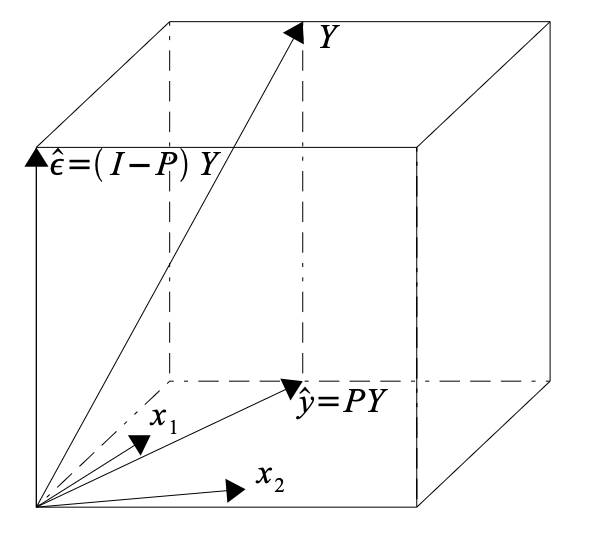
\includegraphics[scale=0.7]{fig/Projektion.png}\\
        Die KQ-Schätzung ist eine orthogonale Projektion von $\bY$ auf den von
        den $\bx$-Vektoren aufgespannten Unterraum.
        \end{minipage}
    };
%------------ Geometrische Interpretation Hat-Matrix und Residualmatrix Header
%---------------------
\node[fill = blue, text=white, font=\bfseries, right=10pt] at (box.north west)
{Geometrische Interpretation};
\end{tikzpicture}


%------------ Eigenschaften der Hat-Matrix und Residualmatrix ---------------
\begin{tikzpicture}
    \node [mybox] (box){%
        \begin{minipage}{0.3\textwidth}
        Die Hat-Matrix $\bP$ und die Residualmatrix $\bQ$ sind
        Projektionsmatrizen und zueinander orthogonal:
        \begin{align*}
        &\bP^\top = \bP \text{ und } \bP^2 = \bP \\
        &\bQ^\top = \bQ \text{ und }  \bQ^2 = \bQ \\
        &\bP\bQ = \bQ\bP = \bm0.
        \end{align*}
        Daraus folgt
        \begin{align*}
        &\V(\hbY) = \ssd \bP \\
        &\V(\hbeps) = \ssd \bQ, \text{ da } \hbeps = \bQ\beps
        \end{align*}
        \end{minipage}
    };
%------------ Eigenschaften der Hat-Matrix und Residualmatrix Header
%---------------------
\node[fill = purple, text=white, font=\bfseries, right=10pt] at (box.north west)
{Eigenschaften von $\bP$ und $\bQ$};
\end{tikzpicture}


%------------ Schätzer für $\ssd$ ---------------
\begin{tikzpicture}
    \node [mybox] (box){%
        \begin{minipage}{0.3\textwidth}
        Gegeben dem multiplen linearen Modell, gilt
        $$\hat{\sd}^2 := \frac{\hbeps^\top\hbeps}{n-p'} = \frac{1}{n-p'}
        \sumin \hat{\eps}_i^2$$ ist ein erwartungstreuer Schätzer von $\ssd$.\\
        \tc{!} Gilt auch ohne die Annahme $\beps \sim \Ncal(\bm0, \ssd \bI)$,
        solange $\E(\beps) = \bm0$ und $\Cov(\beps) = \ssd \bI$
        \end{minipage}
    };
%------------ Schätzer für $\ssd$ Header ---------------------
\node[fill = purple, text=white, font=\bfseries, right=10pt] at (box.north west)
{Schätzer für $\ssd$};
\end{tikzpicture}
    


% %------------ Überschrift ---------------
% \begin{tikzpicture}
%     \node [mybox] (box){%
%         \begin{minipage}{0.3\textwidth}
        
%         \end{minipage}
%     };
% %------------ Überschrifts Header ---------------------
% \node[fill = black, text=white, font=\bfseries, right=10pt] at (box.north west) {Überschrift};
% \end{tikzpicture}
    
\end{multicols*}
\section*{Kapitel 3 - Quadratsummenzerlegung und statistische Inferenz im multiplen linearen Regressionsmodell}

\begin{multicols*}{3}

\tikzstyle{mybox} = [draw=black, fill=white, very thick,
    rectangle, rounded corners, inner sep=10pt, inner ysep=10pt]
\tikzstyle{fancytitle} =[fill=black, text=white, font=\bfseries]



%------------ Quadratsummenzerlegung ---------------
\begin{tikzpicture}
    \node [mybox] (box){%
        \begin{minipage}{0.3\textwidth}
        Gegeben sei das multiple lineare Regressionsmodell mit
        $\rang(\bX) = p'$. Dann gilt
        \footnotesize{
        $$
        \underbrace{(\bY - \bar\bY)^\top (\bY - \bar\bY)}_{SST} =
        \underbrace{(\bY - \hbY)^\top (\bY - \hbY)}_{SSE} + 
        \underbrace{(\hbY - \bar\bY)^\top (\hbY - \bar\bY)}_{SSM}.
        $$}

        \begin{align*}
        & \text{SST(otal):} & & \text{Gesamt-Quadratsumme (korrigiert)}\\
        & \text{SSE(rror):} & &\text{Fehler-Quadratsumme}\\
        & \text{SSM(odel):} & &\text{Modell-Quadratsumme}\\
        \end{align*}
        \end{minipage}
    };
%------------ Quadratsummenzerlegung Header ---------------------
\node[fill = purple, text=white, font=\bfseries, right=10pt] at (box.north west) {Quadratsummenzerlegung};
\end{tikzpicture}
    
\end{multicols*}
\section*{Kapitel 4 - Diskrete Einflußgrößen}

\begin{multicols*}{3}

\tikzstyle{mybox} = [draw=black, fill=white, very thick,
    rectangle, rounded corners, inner sep=10pt, inner ysep=10pt]
\tikzstyle{fancytitle} =[fill=black, text=white, font=\bfseries]



%------------ Kodierung ---------------
\begin{tikzpicture}
    \node [mybox] (box){%
        \begin{minipage}{0.3\textwidth}
        Sei $C$ eine nominale Variable mit $K$ Ausprägungen.
        \vspace{0.5cm}

        \tc{\textbf{Dummy-Kodierung:}}\\
         Wir definieren $K$ neue Variablen $Z_1, \dots, Z_K$ als
         $$Z_k(C) = \begin{cases} 1, & \text{falls } C = k \\ 0, & \text{sonst} \end{cases}$$
         $Z_1, \dots, Z_K$ sind abhängig, da $Z_K = 1 - \sum_{k=1}^{K-1} Z_k$
        \vspace{0.5cm}

        \tc{\textbf{Effekt-Kodierung:}}
        Wir definieren $K-1$ neue Variablen $Z_1^e, \dots, Z_{K-1}^e$ als
        $$Z_k^e(C) = \begin{cases} 1, & \text{falls } C = k \\ -1, & \text{falls } C = K \\ 0, & \text{sonst} \end{cases}$$
        Note: $Z_k(\bC) = \begin{pmatrix}
            Z_k(C_1) \\ \vdots \\ Z_k(C_n) \end{pmatrix}$ und $Z_k^e(\bC) = \begin{pmatrix}
                Z_k^e(C_1) \\ \vdots \\ Z_k^e(C_n) \end{pmatrix}$
    \end{minipage}
    };
%------------ Kodierung Header ---------------------
\node[fill = black, text=white, font=\bfseries, right=10pt] at (box.north west) 
{Kodierung};
\end{tikzpicture}

%------------ Setup einfache Varianzanalyse ---------------
\begin{tikzpicture}
    \node [mybox] (box){%
        \begin{minipage}{0.3\textwidth}
        Im folgenden betrachten wir die einfache Varianzanalyse mit nur einer diskreten Einflußgröße 
        $\bC = \begin{pmatrix} C_1 \\ \vdots \\ C_n \end{pmatrix}$ mit $K$ Ausprägungen.
        Sei $n_k$ dabei die Anzahl der Beobachtungen mit $C_i = k$.
        \end{minipage}
    };
%------------ Setup einfache Varianzanalyse Header ---------------------
\node[fill = black, text=white, font=\bfseries, right=10pt] at (box.north west) 
{Setup einfache Varianzanalyse};
\end{tikzpicture}


%------------ Mittelwertsmodell ---------------
\begin{tikzpicture}
    \node [mybox] (box){%
        \begin{minipage}{0.3\textwidth}
        Das \tc{Mittelwertsmodell} ist gegeben durch
        $$Y_{k_l} = \mu_k + \epsilon_{k_l} \quad l = 1,\dots, n_k \quad k = 1,\dots,K$$
        oder in Matrix-Vektor Notation: 
        $$\bY = (Z_1(\bC) \dotsm Z_K(\bC)) \begin{pmatrix}
            \mu_1 \\ \vdots \\ \mu_K
        \end{pmatrix} + \bepsilon$$
        Bei dem Mittelwertsmodell gibt es keinen Intercept und die $\mu_k$ sind die Mittelwerte der $k$-ten Gruppe.
        Der Effekt der $k$-ten Gruppe ist also $\mu_k$.
        \end{minipage}
    };
%------------ Mittelwertsmodell Header ---------------------
\node[fill = black, text=white, font=\bfseries, right=10pt] at (box.north west) 
{Mittelwertsmodell};
\end{tikzpicture}

%------------ Mittelwertsmodell Beispiel ---------------
\begin{tikzpicture}
    \node [mybox] (box){%
        \begin{minipage}{0.3\textwidth}
        Für $K = 3$ Ausprägungen und $n_k = 2$ für alle $k=1,2,3$ erhalten wir als Mittelwertsmodell:
        $$\bY = \begin{pmatrix} Y_{1_1} \\ Y_{1_2} \\ Y_{2_1} \\ Y_{2_2} \\ Y_{3_1} \\ Y_{3_2}
         \end{pmatrix} = \begin{pmatrix}
            1 & 0 & 0 \\ 1 & 0 & 0 \\ 0 & 1 & 0 \\ 0 & 1 & 0 \\ 0 & 0 & 1 \\ 0 & 0 & 1 \end{pmatrix} \begin{pmatrix}
                \mu_1 \\ \mu_2 \\ \mu_3 \end{pmatrix} + \begin{pmatrix}
                    \eps_{1_1} \\ \eps_{1_2} \\ \eps_{2_1} \\ \eps_{2_2} \\ \eps_{3_1} \\ \eps_{3_2}
        \end{pmatrix}$$
        \end{minipage}
    };
%------------ Mittelwertsmodell Beispiel Header ---------------------
\node[fill = blue, text=white, font=\bfseries, right=10pt] at (box.north west) 
{Mittelwertsmodell Beispiel};
\end{tikzpicture}


%------------ Modell mit Effekt-Kodierung ---------------
\begin{tikzpicture}
    \node [mybox] (box){%
        \begin{minipage}{0.3\textwidth}
        Das \tc{Modell mit Effekt-Kodierung} ist gegeben durch
        $$Y_{k_l} = \mu + \tau_k + \epsilon_{k_l}; \quad \tau_K = -\sum_{k = 1}^{K-1} \tau_k$$ 
        für $\quad l = 1,\dots, n_k \quad k = 1,\dots,K$
        oder in Matrix-Vektor Notation: 
        $$\bY = (\be \hspace{2mm} Z_1^e(\bC) \dotsm Z_{K-1}^e(\bC)) \begin{pmatrix}
            \mu \\ \tau_1 \\ \vdots \\ \tau_{K-1}
        \end{pmatrix} + \bepsilon$$
        Bei dem Modell mit Effekt-Kodierung gibt es einen Intercept $\mu$ und die $\tau_k$ sind die Abweichungen der $k$-ten Gruppe vom Gesamtmittelwert bzw. vom Intercept $\mu$.
        Der Effekt der $k$-ten Gruppe ist also $\mu + \tau_k$.
        \end{minipage}
    };
%------------ Modell mit Effekt-Kodierung Header ---------------------
\node[fill = black, text=white, font=\bfseries, right=10pt] at (box.north west) 
{Modell mit Effekt-Kodierung};
\end{tikzpicture}

%------------ Modell mit Effekt-Kodierung Beispiel ---------------
\begin{tikzpicture}
    \node [mybox] (box){%
        \begin{minipage}{0.3\textwidth}
        Für $K = 3$ Ausprägungen und $n_k = 2$ für alle $k=1,2,3$ erhalten wir als Modell mit Effekt-Kodierung:
        $$\bY = \begin{pmatrix} Y_{1_1} \\ Y_{1_2} \\ Y_{2_1} \\ Y_{2_2} \\ Y_{3_1} \\ Y_{3_2}
         \end{pmatrix} = \begin{pmatrix}
            1 & 1 & 0 \\ 1 & 1 & 0 \\ 1 & 0 & 1 \\ 1 & 0 & 1 \\ 1 & -1 & -1 \\ 1 & -1 & -1 \end{pmatrix} \begin{pmatrix}
                \mu \\ \tau_1 \\ \tau_2  \end{pmatrix}
         + \begin{pmatrix}
            \eps_{1_1} \\ \eps_{1_2} \\ \eps_{2_1} \\ \eps_{2_2} \\ \eps_{3_1} \\ \eps_{3_2} \end{pmatrix}$$
                \end{minipage}
    };
%------------ Modell mit Effekt-Kodierung Beispiel Header ---------------------
\node[fill = blue, text=white, font=\bfseries, right=10pt] at (box.north west) 
{Modell mit Effekt-Kodierung Beispiel};
\end{tikzpicture}

%------------ Modell mit Referenz-Kodierung ---------------
\begin{tikzpicture}
    \node [mybox] (box){%
        \begin{minipage}{0.3\textwidth}
        Das \tc{Modell mit Referenz-Kodierung} ist gegeben durch
        $$Y_{k_l} = \mu_K + \tau_k + \epsilon_{k_l}; \quad \tau_K = 0$$ 
        für $\quad l = 1,\dots, n_k \quad k = 1,\dots,K$
        oder in Matrix-Vektor Notation:
        $$\bY = (\be \hspace{2mm} Z_1(\bC) \dotsm Z_{K-1}(\bC)) \begin{pmatrix}
            \mu_K \\ \tau_1 \\ \vdots \\ \tau_{K-1}
        \end{pmatrix} + \bepsilon$$
        Beim Modell mit Referenz-Kodierung gibt es einen Intercept $\mu_K$ der den Mittelwert der $K$-ten Gruppe angibt und die $\tau_k$ sind die Abweichungen der $k$-ten Gruppe vom Mittelwert der $K$-ten Referenz-Gruppe.
        Der Effekt der $k$-ten Gruppe ist also $\mu_K + \tau_k$ für $k = 1,\dots,K-1$ und $\mu_K$ für $k = K$.
        \end{minipage}
    };
%------------ Modell mit Referenz-Kodierung Header ---------------------
\node[fill = black, text=white, font=\bfseries, right=10pt] at (box.north west) 
{Modell mit Referenz-Kodierung};
\end{tikzpicture}

%------------ Modell mit Referenz-Kodierung Beispiel ---------------
\begin{tikzpicture}
    \node [mybox] (box){%
        \begin{minipage}{0.3\textwidth}
        Für $K = 3$ Ausprägungen und $n_k = 2$ für alle $k=1,2,3$ erhalten wir als Modell mit Referenz-Kodierung:
        $$\bY = \begin{pmatrix} Y_{1_1} \\ Y_{1_2} \\ Y_{2_1} \\ Y_{2_2} \\ Y_{3_1} \\ Y_{3_2}
         \end{pmatrix} = \begin{pmatrix}
            1 & 1 & 0 \\ 1 & 1 & 0 \\ 1 & 0 & 1 \\ 1 & 0 & 1 \\ 1 & 0 & 0 \\ 1 & 0 & 0 \end{pmatrix} \begin{pmatrix}
                \mu_3 \\ \tau_1 \\ \tau_2  \end{pmatrix}
         + \begin{pmatrix}
            \eps_{1_1} \\ \eps_{1_2} \\ \eps_{2_1} \\ \eps_{2_2} \\ \eps_{3_1} \\ \eps_{3_2} \end{pmatrix}$$
                \end{minipage}
    };
%------------ Modell mit Referenz-Kodierung Beispiel Header ---------------------
\node[fill = blue, text=white, font=\bfseries, right=10pt] at (box.north west) 
{Modell mit Referenz-Kodierung Beispiel};
\end{tikzpicture}

%------------ Bemerkungen-Kodierung ---------------
\begin{tikzpicture}
    \node [mybox] (box){%
        \begin{minipage}{0.3\textwidth}
        Alle Modellvarianten führen zur gleichen Modellanpassung ($R^2$).
        Die Parameter haben aber unterschiedliche Interpretationen. Parameter und deren Schätzer sind aber ineinander umrechenbar.
        \end{minipage}
    };
%------------ Bemerkungen-Kodierung Header ---------------------
\node[fill = purple, text=white, font=\bfseries, right=10pt] at (box.north west) 
{Bemerkungen-Kodierung};
\end{tikzpicture}

\newpage

%------------ Setup einfache Varianzanalyse ---------------
\begin{tikzpicture}
    \node [mybox] (box){%
        \begin{minipage}{0.3\textwidth}
        Im folgenden betrachten wir zwei diskrete Einflußgrößen $\bC = \begin{pmatrix} C_1 \\ \vdots \\ C_n \end{pmatrix}$ und 
        $\bD = \begin{pmatrix} D_1 \\ \vdots \\ D_n \end{pmatrix}$ mit $K_C$ bzw. $K_D$ Ausprägungen.
        Sei $n_{k,l}$ dabei die Anzahl der Beobachtungen mit $C_i = k$ und $D_j = l$.\\
        \vspace{1mm}

        \tc{!} Hier ist die Mittelwertsdarstellung bzw. das Mittelwertsmodell nicht möglich, da dieser davon abhängig ist, welche Variable zuerst kodiert wird.
        \end{minipage}
    };
%------------ Setup einfache Varianzanalyse Header ---------------------
\node[fill = black, text=white, font=\bfseries, right=10pt] at (box.north west) 
{Setup zweifaktorielle Varianzanalyse};
\end{tikzpicture}

%------------ Modell mit Effekt-Kodierung (mehrfaktoriell) ---------------
\begin{tikzpicture}
    \node [mybox] (box){%
        \begin{minipage}{0.3\textwidth}
        Das \tc{Modell mit Effekt-Kodierung} ist gegeben durch
        $$\bY = (\be \hspace{2mm} Z_1^e(\bC) \dotsm Z_{K-1}^e(\bC)) \begin{pmatrix}
            \mu \\ \tau_1 \\ \vdots \\ \tau_{K-1}
        \end{pmatrix} + \bepsilon$$
        Bei dem Modell mit Effekt-Kodierung gibt es einen Intercept $\mu$ und die $\tau_k$ sind die Abweichungen der $k$-ten Gruppe vom Gesamtmittelwert bzw. vom Intercept $\mu$.
        Der Effekt der $k$-ten Gruppe ist also $\mu + \tau_k$.
        \end{minipage}
    };
%------------ Modell mit Effekt-Kodierung (mehrfaktoriell) Header ---------------------
\node[fill = black, text=white, font=\bfseries, right=10pt] at (box.north west) 
{Modell mit Effekt-Kodierung (mehrfaktoriell)};
\end{tikzpicture}

\end{multicols*}
\section*{Kapitel 5 - Metrische Einflußgrößen}

\begin{multicols*}{3}

\tikzstyle{mybox} = [draw=black, fill=white, very thick,
    rectangle, rounded corners, inner sep=10pt, inner ysep=10pt]
\tikzstyle{fancytitle} =[fill=black, text=white, font=\bfseries]



%------------ Interaktion metrischer Variablen ---------------
\begin{tikzpicture}
    \node [mybox] (box){%
        \begin{minipage}{0.3\textwidth}
        Seien $X_1, X_2$ zwei metrische Variablen mit den Ausprägungen $x_{1i}, x_{2i}$ für $i = 1, \dots, n$.
        Die Modellgleichung für das Modell mit Interaktion 
        lautet:
        \begin{align*}
            Y_i &= \beta_0 + \beta_1 x_{1i} + \beta_2 x_{2i} + \beta_3 x_{1i} x_{2i} + \epsilon_i\\
                &= \beta_0 + \beta_2 x_{2i} + (\beta_1 + \beta_3 x_{2i})x_{1i}  + \epsilon_i\\
                &= \beta_0 + \beta_1 x_{1i} + (\beta_2 + \beta_3 x_{1i})x_{2i}  + \epsilon_i
        \end{align*}

        Interpreation der Modellparameter:\\
        Die Parameter $\gb{1}, \gb{2}$ geben die Steigung bei $x_1 = x_2 = 0$ an. I.d.R.
        nicht sinnvoll interpretierbar.
        

    \end{minipage}
    };
%------------ Interaktion metrischer Variablen Header ---------------------
\node[fill = black, text=white, font=\bfseries, right=10pt] at (box.north west) 
{Interaktion metrischer Variablen};
\end{tikzpicture}

%------------ Modelle mit metrischen Variablen ---------------
\begin{tikzpicture}
    \node [mybox] (box){%
        \begin{minipage}{0.3\textwidth}
        Sei $X$ eine metrische Variable mit den Ausprägungen $x_{i}$ für $i = 1, \dots, n$. Typische Modelle sind:
        \begin{itemize}
            \item \textbf{Einfaches lineares Modell:} \\
            $Y_i = \beta_0 + \beta_1 x_{i} + \epsilon_i$
            \item \textbf{Transformiertes lineares Modell:} \\
            $Y_i = \beta_0 + \beta_1 T(x_{i}) + \epsilon_i$, \quad z.B. $T(x) = \log(x)$
            \item \textbf{Polynomielles Modell:} \\
            $Y_i = \beta_0 + \beta_1 x_{i} + \beta_2 x_{i}^2 + \dots + \beta_d x_{i}^d + \epsilon_i$\\
            Problem: Bestimmung von $d$.\\
            Mögliche Lösung: Test auf Signifikanz der Koeffizienten $\gb{2},
            \dots, \gb{d}$ mittels sequentieller Quadratsummenzerlegung.
            \item \textbf{Stückweise konstantes Modell:} \\
            $Y_i = \beta_0 I_{[x_{i} \leq g_1]} + \beta_1 I_{[g_1 < x_{i} \leq
            g_2]} + \dots + \beta_{k-1} I_{[g_{k-1} < x_{i} \leq g_k]} +
            \beta_{p} I_{[x_{i} > g_p]} + \epsilon_i$\\
            Dies entspricht der Kategorisierung der x-Variablen.
            \item \textbf{Stückweise lineares Modell:} \\
            $Y_i = \beta_0 + \beta_1 x_{i} + \beta_2 \max\{x_i-g_1, 0\} + \dots
            + \beta_{p} \max\{x_i-g_{h}, 0\} + \epsilon_i$\\
            mit bekannten Bruchpunkten (Knoten) $g_j$.
            \item \textbf{Regressionssplines:} \\
            $Y_i = \beta_0 + \beta_1 x_{i} + \beta_2 x_i^2 + \dots + \beta_{k}
            x_i^{k} + \beta_{k + 1} \max\{x_i - g_1, 0\}^3 + \dots + \beta_{k +
            h} \max\{x_i - g_h, 0\}^3 + \epsilon_i$\\
            Ein Polynom 3.Grades ist 2-mal stetig differenzierbar.
        \end{itemize}
        

    \end{minipage}
    };
%------------ Modelle mit metrischen Variablen Header ---------------------
\node[fill = blue, text=white, font=\bfseries, right=10pt] at (box.north west) 
{Modelle mit metrischen Variablen};
\end{tikzpicture}


%------------ Allgemeiner Ansatz mit Basisfunktionen ---------------
\begin{tikzpicture}
    \node [mybox] (box){%
        \begin{minipage}{0.3\textwidth}
        Sei $X$ eine metrische Variable mit den Ausprägungen $x_{i}$ für $i = 1, \dots, n$.\\
        Allgemeiner Ansatz für Modelle mit Basisfunktionen:\\
        Seien $B_1, B_2, \dots, B_k$ Basisfunktionen. Dann ist die allgemeine Modellgleichung:
        \begin{align*}
            Y_i &= \beta_0 + \beta_1 B_1(x_{i}) + \beta_2 B_2(x_{i}) + \dots + \beta_k B_k(x_{i}) + \epsilon_i
        \end{align*}

    \end{minipage}
    };
%------------ Allgemeiner Ansatz mit Basisfunktionen Header ---------------------
\node[fill = purple, text=white, font=\bfseries, right=10pt] at (box.north west) 
{Allgemeiner Ansatz mit Basisfunktionen};
\end{tikzpicture}


\end{multicols*}
\section*{Kapitel 6 - Modelldiagnose}

\begin{multicols*}{3}

\tikzstyle{mybox} = [draw=black, fill=white, very thick,
    rectangle, rounded corners, inner sep=10pt, inner ysep=10pt]
\tikzstyle{fancytitle} =[fill=black, text=white, font=\bfseries]



%------------ Arten von Residuen ---------------
\begin{tikzpicture}
    \node [mybox] (box){%
        \begin{minipage}{0.3\textwidth}
        Gegeben sei das multiple lineare Regressionsmodell mit den üblichen Annahmen über $\beps$ und $\bX$.
        Aus Kapitel 2 wissen wir, dass $\V(\hbeps) = \sigma^2 \bQ$ und somit $\V(\hat{\eps_i}) = \sigma^2 q_{ii}$,
        wobei $q_{ii}$ das $i$-te Diagonalelement der Matrix $\bQ$ ist.

        Wir definieren \tc{standardisierte Residuen} als
        \begin{align*}
            r_i &= \frac{\hat{\eps_i}}{\sqrt{\hat{\sigma}^2 q_{ii}}}
        \end{align*}
        
        Das Problem an den standardisierten Residuen ist, dass bei der Schätzung
        von $\sigma^2$ die Residuen mit einbezogen werden. Dies führt zu einer
        Verzerrung der Residuen. Wir definieren daher zusätzlich
        \tc{studentisierte Residuen} als

        \begin{align*}
            r_i^* &= \frac{\hat{\eps_i}}{\sqrt{\hat{\sigma}_{(i)}^2 q_{ii}}}\\
            & = r_i \sqrt{\frac{n-p-1}{n-p-r_i^2}} \sim t_{n-p-1}
        \end{align*}
        wobei $\hat{\sigma}_{(i)}^2$ die Schätzung von $\sigma^2$ ist, die ohne die $i$-te
        Beobachtung berechnet wurde.
        Man kann zeigen, dass die studentisierten Residuen $t$-verteilt sind.

        Wir können 

    \end{minipage}
    };
%------------ Arten von Residuen Header ---------------------
\node[fill = black, text=white, font=\bfseries, right=10pt] at (box.north west) 
{Arten von Residuen};
\end{tikzpicture}

%------------ Durbin-Watson-Test ---------------
\begin{tikzpicture}
    \node [mybox] (box){%
        \begin{minipage}{0.3\textwidth}
        
        Wir definieren die \tc{Durbin-Watson-Teststatistik} als
        $$d := \frac{\sum_{i = 2}^{n} (\hat{\eps}_i - \hat{\eps}_{i-1})^2}{\sumin \hat{\eps}_i^2} \approx 2(1-\hat{\rho})$$
        wobei $\hat{\rho}$ die Korrelation zwischen $\hat{\eps}_i$ und $\hat{\eps}_{i-1}$ beschreibt.

        Die Verteilung von $d$ unter $H_0: \rho = 0$ ist schwierig allgemein herzuleiten.
        Es gilt heuristisch, dass wir $H_0$ verwerfen, wenn $d \approx 2$

        Für genaue Tests können wir in R aus dem package $\tt{lmtest}$ die Funktion $\tt{dwtest}$ nutzen.


    \end{minipage}
    };
%------------ Durbin-Watson-Test Header ---------------------
\node[fill = purple, text=white, font=\bfseries, right=10pt] at (box.north west) 
{Durbin-Watson-Test};
\end{tikzpicture}



%------------ Mögliche Probleme ---------------
\begin{tikzpicture}
    \node [mybox] (box){%
        \begin{minipage}{0.3\textwidth}
        Gegeben sei das multiple lineare Regressionsmodell mit den üblichen Annahmen über $\beps$ und $\bX$.
        Folgende Probleme können typischerweise auftreten:

        \begin{itemize}
            \item \textbf{$\eps_i$ nicht normalverteilt:} \\
            Die Fehlerterme sind nicht normalverteilt.
            \item \textbf{Heteroskedastizität:} \\
            Die Varianz der Fehlerterme ist nicht konstant bzw. von $i$ abhängig.
            \item \textbf{Autokorrelation:} \\
            Die Fehlerterme sind korreliert.
            \item \textbf{Multikollinearität:} \\
            Die Kovariablen sind (annähernd) linear abhängig.
            \item \textbf{Ausreißer und Leverage Points:} \\
            Einzelne Beobachtungen haben einen starken Einfluss auf die Schätzungen.
            \item \textbf{Overfitting oder Underfitting:} \\
            Das Modell ist zu komplex oder zu einfach bzw. die Modellgleichung ist fehlerhaft.
        \end{itemize}

    \end{minipage}
    };
%------------ Mögliche Probleme Header ---------------------
\node[fill = black, text=white, font=\bfseries, right=10pt] at (box.north west) 
{Mögliche Probleme};
\end{tikzpicture}

%------------ Mögliche Probleme 1 ---------------
\begin{tikzpicture}
    \node [mybox] (box){%
        \begin{minipage}{0.3\textwidth}

        \begin{itemize}
            \item \textbf{Ursachen}: Die abhängige Variable $Y$ kann bedingt auf
            $\bx$ nicht normalverteilt sein. Das ist z.B. der Fall, wenn $Y$
            eine Zählgröße, eine Überlebenszeit, ein Anteil, nicht-negativ oder
            eine binäre Variable ist.
            \item \textbf{Folgen}: KQ-Schätzer bleibt unbiased und F-Statistik ist i.A.
            robust. Aber Konfidenz-/Prognoseintervalle sind nicht mehr korrekt.
            \item \textbf{Diagnose}: Schiefe, Kurtosis, Normal-Plot der Residuen.
            \item \textbf{Therapie}: Transformation der abhängigen Variable $Y$. GLMs.
        \end{itemize}

    \end{minipage}
    };
%------------ Mögliche Probleme 2 Header ---------------------
\node[fill = blue, text=white, font=\bfseries, right=10pt] at (box.north west) 
{$\eps_i$ nicht normalverteilt};
\end{tikzpicture}

%------------ Heteroskedastizität ---------------
\begin{tikzpicture}
    \node [mybox] (box){%
        \begin{minipage}{0.3\textwidth}

        \begin{itemize}
            \item \textbf{Ursachen}: Die abhängige Variable $Y$ stellt z.B. eine
            Zählgröße oder Anteil dar. Gruppierte Daten führen zu verschieden
            Residualvarianzen innerhalb der Gruppen. Multiplikative
            Fehlerstruktur, d.h. $\ssd_i$ ist abhängig von der Größe von $Y_i$ .
            \item \textbf{Folgen}: KQ-Schätzer bleibt unbiased, aber ist nicht mehr most
            efficient. Tests und Konfidenz-/Prognoseintervalle sind nicht mehr
            korrekt.
            \item \textbf{Diagnose}: Residuals vs. Fitted Plot. Berechnung der
            Residualvarianzen in den einzelnen Gruppen (bei gruppierten Daten).
            \item \textbf{Therapie}: Transformation der abhängigen Variable $Y$.
            Gewichtete KQ-Schätzung.
        \end{itemize}

    \end{minipage}
    };
%------------ Heteroskedastizität Header ---------------------
\node[fill = blue, text=white, font=\bfseries, right=10pt] at (box.north west) 
{Heteroskedastizität};
\end{tikzpicture}


%------------ Autokorrelation ---------------
\begin{tikzpicture}
    \node [mybox] (box){%
        \begin{minipage}{0.3\textwidth}

        \begin{itemize}
            \item \textbf{Ursachen}: Zeitreihenstruktur oder räumliche Struktur
            der Daten führen zu positiver Korrelation von aufeinander folgenden
            (bzw. nahen) Beobachtungen. Residuen bei gruppierten Beobachtungen,
            bei denen die Gruppenzugehörigkeit nicht zusätzlich modelliert wird,
            sind häufig positiv korreliert.
            \item \textbf{Folgen}: KQ-Schätzer bleibt unbiased, aber ist nicht mehr most
            efficient. Tests und Konfidenz-/Prognoseintervalle sind nicht mehr
            korrekt.
            \item \textbf{Diagnose}: Analyse der Zeitreihenstruktur der
            Residuen, z.B. mit Durbin-Watson-Test; Plots der Residuen gegen die
            Zeit; Plots von $\hat{\eps}_i$ gegen $\hat{\eps}_{i-1}$. ACP und PACP.
            \item \textbf{Therapie}: Verwendung von Zeitreihenmethoden;
            Einbeziehung von Trend und Saison; Gewichtete KQ-Methode.

        \end{itemize}

    \end{minipage}
    };
%------------ Autokorrelation Header ---------------------
\node[fill = blue, text=white, font=\bfseries, right=10pt] at (box.north west) 
{Autokorrelation};
\end{tikzpicture}


%------------ Multikollinearität ---------------
\begin{tikzpicture}
    \node [mybox] (box){%
        \begin{minipage}{0.3\textwidth}

        \begin{itemize}
            \item \textbf{Ursachen}: Hohe Korrelation zwischen den Einflussgrößen; Ungünstiges
            Versuchs-Design; Codierung von diskreten Variablen.
            \item \textbf{Folgen}: Ungenauer KQ-Schätzer, häufig sogar mit falschem Vorzeichen. Aber
            Konfidenzintervalle sind korrekt (jedoch entsprechend sehr breit).
            \item \textbf{Diagnose}: Analyse der Matrix $\bX^\top \bX$ und der Korrelationsmatrix der
            metrischen Einflussgrößen.
            \begin{itemize}
                \item Konditionszahl von $\bX$: 
                $$\kappa(\bX) = \sqrt{\frac{\lambda_{max}(\bX^\top
                \bX)}{\lambda_{min}(\bX^\top \bX)}}$$
                $\kappa(\bX) \gg 1$ deutet auf Multikollinearität hin.
                \item Varianz Inflationsfaktor: $$\V(\hbe{j}) =
                \frac{\sigma^2}{(1-R_j^2) \sumin (x_{ij} - \overline{\bx_j})},$$
                wobei $R_j^2$ das Bestimmheitsmaß der Regression $\bX_j =
                \bX_{-j}\mathbf{\alpha} + \mathbf{\delta}$ ist. Wir definieren
                den \tc{Varianz Inflationsfaktor} als $$VIF_j =
                \frac{1}{1-R_j^2}.$$ Wenn $VIF_j = 1$, dann heißt das, dass
                $\bX_j$ orthogonal zu allen anderen Regressoren ist. Ein hohes
                $VIF_j$ deutet auf Multikollinearität hin. Als Heuristik wird
                oft $VIF_j > 10$ als kritisch angesehen.
                
            \end{itemize}
            \item \textbf{Therapie}: Zusammenfassen bzw. Weglassen von
            Einflussgrößen; Verwendung von anderen Schätzmethoden, z.B.:
            Ridge-Regression.
        \end{itemize}

    \end{minipage}
    };
%------------ Multikollinearität Header ---------------------
\node[fill = blue, text=white, font=\bfseries, right=10pt] at (box.north west) 
{Multikollinearität};
\end{tikzpicture}


%------------ Ausreißer und Leverage Points ---------------
\begin{tikzpicture}
    \node [mybox] (box){%
        \begin{minipage}{0.3\textwidth}
        Wir unterscheiden zwischen Ausreißern und High Leverage Points
        (einflußreiche Beobachtungen). Ein \tc{Ausreißer} ist eine Beobachtung,
        die in der abhängigen Variable $Y$ stark von den anderen Beobachtungen
        abweicht (i.d.R. hoher Störterm). Ein \tc{Leverage Point} ist eine
        Beobachtung, die in den unabhängigen Variablen $\bX$ stark von den
        anderen Beobachtungen abweicht.
        \begin{itemize}
            \item \textbf{Ursachen}: Falsche Erhebung; Beobachtung gehört
            nicht zur Grundgesamtheit; Besonderheiten bei einzelner
            Untersuchungseinheit.
            \item \textbf{Folgen}: High Leverage Points haben einen großen
            Einfluss auf $\hbbeta$. Ausreißer können zu erheblicher Verzerrung
            von $\hbbeta$ führen.
            \item \textbf{Diagnose}: Analyse der Diagonalelemente der Hat-Matrix
            $\bP$ zum Auffinden von high leverage points; Verschiedene Residuenplots
            zur Ausreißeranalyse; Influence-Statistiken.
            \item \textbf{Therapie}: Fehlerhafte Daten weglassen
            (Sensitivitätsanalyse); Robuste Regression; Gewichtete Regression.

        \end{itemize}

        Wir definieren \tc{Leverage} als
        \begin{align*}
            h_{ii} &= \bP_{ii} = \frac{\V(\hbY_i)}{\ssd} \\
            &=\bx_i^\top (\bX^\top \bX)^{-1} \bx_i = \lVert \bx_i \rVert^2_{(\bX^\top \bX)^{-1}}
        \end{align*}
        Optimalerweise gilt $h_{ii} = \frac{p'}{n}$ und 
        als Heuristik wird oft $h_{ii} > \frac{2p'}{n}$ als kritisch angesehen.\\
        \tc{!} Der Leverage kann nach Transformation auch als quadratischer
        Mahalanobis-Abstand zum Mittelpunkt interpretiert werden.
        
        Wir definieren \tc{Cook's Distanz} als
        \begin{align*}
            D_i &:= \frac{(\hbbeta_{-i} - \hbbeta)^\top (\bX^\top \bX)
            (\hbbeta_{-i} - \hbbeta)}{\hssd p'} \\
            &= \frac{(\hbY_{-i} - \hbY)^\top
            (\hbY_{-i} - \hbY)}{\hssd p'} \\
            &= \frac{r_i^2}{p'} \cdot \frac{h_{ii}}{1-h_{ii}}
        \end{align*}
        Als Heuristik wird oft verwendet, dass Beobachtungen mit $D_i > 0.5$
        auffällig sind und Beobachtungen mit $D_i > 1$ auf jeden Fall untersucht
        werden sollten.
    \end{minipage}
    };
%------------ Ausreißer und Leverage Points Header ---------------------
\node[fill = blue, text=white, font=\bfseries, right=10pt] at (box.north west) 
{Ausreißer und Leverage Points};
\end{tikzpicture}

%------------ Overfitting oder Underfitting ---------------
\begin{tikzpicture}
    \node [mybox] (box){%
        \begin{minipage}{0.3\textwidth}

        \begin{itemize}
            \item \textbf{Ursachen}: Variablen wurden weggelassen oder
            überflüssigerweise in das Modell einbezogen; Der Zusammenhang ist
            nicht linear; Interaktionen werden nicht in das Modell einbezogen.

            \item \textbf{Folgen}: Systematische Fehler bei der Schätzung der
            Modellparameter und bei der Prognose; Dennoch: Modellschätzung
            liefert häufig brauchbare Näherung.

            \item \textbf{Diagnose}: Residuenplots $\hbeps$ gegen $\hbY$;
            F-Tests auf Einfluss von weiteren Variablen; Interaktionen;
            Polynomterme höherer Ordnung, etc.

            \item \textbf{Therapie}: Modellerweiterung; Transformationen der
            Einflussgrößen; Variablenselektionsverfahren (z.B. LASSO).

        \end{itemize}

    \end{minipage}
    };
%------------ Overfitting oder Underfitting Header ---------------------
\node[fill = blue, text=white, font=\bfseries, right=10pt] at (box.north west) 
{Overfitting oder Underfitting};
\end{tikzpicture}



\end{multicols*}
\section*{Kapitel 7 - Fortgeschrittenere lineare Modelle}

\begin{multicols*}{3}

\tikzstyle{mybox} = [draw=black, fill=white, very thick,
    rectangle, rounded corners, inner sep=10pt, inner ysep=10pt]
\tikzstyle{fancytitle} =[fill=black, text=white, font=\bfseries]



%------------ Das Allgemeine lineare Regressionsmodell ---------------
\begin{tikzpicture}
    \node [mybox] (box){
    \begin{minipage}{0.3\textwidth}
    Das \tc{allgemeine lineare Regressionsmodell} hat die Form
    $$\bY = \bX\bbeta + \beps,$$ wobei wir nun annehmen, dass $\beps \sim
    \Ncal(\bf0, \ssd \bW^{-1})$, mit \textbf{bekannter} positiv definiter Matrix $\bW$. Wir nennen
    $\bW$ die \tc{Gewichtsmatrix}.

    Im Falle von heteroskedastischen, aber unkorrelierten Fehlern ist $\bW$ eine
    Diagonalmatrix mit $\bW = \diag(w_1, \cdots, w_n)$ und $\V(\beps) = 
    \diag(\frac{\ssd}{w_1}, \cdots, \frac{\ssd}{w_n})$.
    \end{minipage}
    };
%------------ Das Allgemeine lineare Regressionsmodell Header ---------------------
\node[fill = black, text=white, font=\bfseries, right=10pt] at (box.north west) 
{Das allgemeine lineare Regressionsmodell};
\end{tikzpicture}

%------------ Schätzer im allgemeinen lineare Regressionsmodell ---------------
\begin{tikzpicture}
    \node [mybox] (box){
    \begin{minipage}{0.3\textwidth}
    Gegeben sei das \tc{allgemeine lineare Regressionsmodell}
    $\bY = \bX\bbeta + \beps$ mit $\beps \sim \Ncal(\bf0, \ssd \bW^{-1})$.

    Dann gilt:
    \begin{align*}
        \hbbeta &= (\bX^\top\bW\bX)^{-1}\bX^\top\bW\bY,\\
        \E(\hbbeta) &= \bbeta,\\
        \V(\hbbeta) &= \ssd(\bX^\top\bW\bX)^{-1}
    \end{align*}
    und $\hbbeta$ ist der \tc{Beste lineare unverzerrte Schätzer} (BLUE) für $\bbeta$.
    
    Der \tc{Schätzer für $\ssd$} ist gegeben durch den REML-Schätzer
    $$\hssd = \frac{\hbeps^\top \bW \hbeps}{n - p'},$$

    \tc{!} Alle Schätzer setzen voraus, dass $\bW$ bekannt ist.

    \end{minipage}
    };
%------------ Schätzer im allgemeinen lineare Regressionsmodell Header ---------------------
\node[fill = purple, text=white, font=\bfseries, right=10pt] at (box.north west) 
{Schätzer im allg. linearen Regressionsmodell};
\end{tikzpicture}

%------------ Umformung ---------------
\begin{tikzpicture}
    \node [mybox] (box){
    \begin{minipage}{0.3\textwidth}
    Wir können die symmetrische positiv definite Gewichtsmatrix $\bW$
    zerlegen durch $$\bW = \bV\bD\bV^\top,$$ wobei $\bD$ eine Diagonalmatrix
    ist.
    Dann definieren wir $\bW^{\frac{1}{2}} = \bV\bD^{\frac{1}{2}}\bV^\top$.
    Mit dieser Zerlegung können wir das allgemeine lineare Regressionsmodell
    in ein klassisches lineares Regressionsmodell umformen durch
    $$\bY^* = \bX^*\bbeta^* + \beps^*, \quad \beps^* \sim \Ncal(\bf0, \ssd \bI)$$ wobei
    $$\bY^* = \bW^{\frac{1}{2}}\bY, \quad \bX^* = \bW^{\frac{1}{2}}\bX, \quad
    \beps^* = \bW^{\frac{1}{2}}\beps.$$

    \end{minipage}
    };
%------------ Umformung Header ---------------------
\node[fill = purple, text=white, font=\bfseries, right=10pt] at (box.north west) 
{Umformung};
\end{tikzpicture}

%------------ AR(1) Modell ---------------
\begin{tikzpicture}
    \node [mybox] (box){
    \begin{minipage}{0.3\textwidth}
    
    Das \tc{AR(1) Zeitreihenmodell} hat die Form
    $$\eps_t = \phi \eps_{t-1} + \eta_t, \quad t = 2,\dots,n$$ wobei $\eta_t
    \sim \Ncal(0, \sigma^2), |\phi| < 1$ und $\V(\eps_1) = \frac{\ssd}{1-\phi^2}$.

    Dann ist die Kovarianzmatrix $\bW^{-1}$ gegeben durch
    $$\bW^{-1} = \frac{1}{1 - \phi^2} \begin{pmatrix}
        1 & \phi & \phi^2 & \cdots & \phi^{n-1}\\
        \phi & 1 & \phi & \cdots & \phi^{n-2}\\
        \phi^2 & \phi & 1 & \cdots & \phi^{n-3}\\
        \vdots & \vdots & \vdots & \ddots & \vdots\\
        \phi^{n-1} & \phi^{n-2} & \phi^{n-3} & \cdots & 1
    \end{pmatrix}$$
    Damit gilt also
    $$\beps \sim \Ncal(\bf0, \ssd \bW^{-1}).$$

    \end{minipage}
    };
%------------ AR(1) Header ---------------------
\node[fill = blue, text=white, font=\bfseries, right=10pt] at (box.north west) 
{AR(1) Zeitreihenmodell};
\end{tikzpicture}

%------------ Linear Mixed Modell ---------------
\begin{tikzpicture}
    \node [mybox] (box){
    \begin{minipage}{0.3\textwidth}

    Wir betrachten die Beobachtungen $(Y_{ij}, \bx_{ij}^\top)$ mit $i =
    1,\dots,K$ und $j = 1,\dots,n_i$.
    
    In der Regel benutzen wir dieses Setting in zwei Fällen:
    \begin{enumerate}
        \item Clustered Data: $i$ beschreibt eine Gruppe und $j$ ein Objekt
        innerhalb dieser Gruppe (z.B. Schüler $j$ in einer Klasse $i$).
        \item Longitudinal Data: $i$ beschreibt eine Untersuchungseinheit und
        $j$ ein Beobachtung dieser Untersuchungseinheit zum Zeitpunkt $t_{ij}$
        (z.B. Messung von Patient $i$ zum Zeitpunkt $t_{ij}$).
    \end{enumerate}
    
    Die Idee eines \tc{Linear Mixed Modells} ist, dass wir ein Cluster-übergreifendes
    bzw. Untersuchungseinheiten-übergreifendes Modell haben, aber innerhalb der
    Cluster bzw. Untersuchungseinheiten können die Beobachtungen korreliert sein und
    zufällig vom übergreifenden Modell abweichen.

    
\end{minipage}
};
%------------ Linear Mixed Modell Header ---------------------
\node[fill = black, text=white, font=\bfseries, right=10pt] at (box.north west) 
{Linear Mixed Modell};
\end{tikzpicture}

%------------ Linear Mixed Modell ---------------
\begin{tikzpicture}
    \node [mybox] (box){
    \begin{minipage}{0.3\textwidth}

    Das \tc{Random Intercept Modell} ist definert durch
    $$Y_{ij} = \bx_{ij}^\top\bbeta + \gamma_{0i} + \eps_{ij}, \quad i =
    1,\dots,K, \quad j = 1,\dots,n_i$$ mit $\eps_{ij} \sim \Ncal(0,\ssd),
    i.i.d.$ und $\gamma_{0i} \sim \Ncal(0, \ssd_{\gamma_0}), i.i.d.$ und
    $\sum_{i = 1}^{K} n_i = n$ und der Annahme, dass die $\eps_{ij}$ unabhängig
    von den $\gamma_{0i}$ sind.\\

    Wir bezeichnen $\beta_0$ als den fixed Population Intercept und
    $\gamma_{0i}$ als die Cluster-spezifische bzw.
    Untersuchungseinheiten-spezifische zufällige Abweichung vom fixed Population
    Intercept. Zusammen bezeichnen wir $\beta_0 + \gamma_{0i}$ als den
    \tc{random Intercept} von Cluster/Untersuchungseinheit $i$. Die restlichen
    $\beta_j$ sind die \tc{fixed Effekte}.\\

    Zwischen den Cluster/Untersuchungseinheiten sind die $Y_{ij}$ unabhängig
    und es gilt das konditionalle Modell für $i = 1,\dots,K$
    $$Y_{ij}\mid \gamma_{0i} \sim \Ncal(\bx_{ij}^\top\bbeta + \gamma_{0i},
    \ssd).$$

    Innerhalb eines Clusters/Untersuchungseinheit sind die $Y_{ij}$ korreliert.
    Wir bezeichnen diese Korrelation als \tc{Intra-Class Correlation} (ICC). Es gilt
    $$\corr(Y_{ij}, Y_{il})= \frac{\ssd_{\gamma_0}}{\ssd_{\gamma_0} + \ssd}, \quad j,l = 1,\dots,n_i, j\neq l$$
    und
    $$\V(\bY_i) = \ssd\bI_{n_i} + \ssd_{\gamma_0} \bJ_{n_i}, \quad i = 1,\dots,K$$
    wobei $\bJ_{n_i}$ die $n_i \times n_i$-Matrix mit Einsen ist.

    Daraus ergibt sich das \tc{marginale Modell}
    $$\bY_i \sim \Ncal(\bX_i\bbeta, \ssd\bI_{n_i} + \ssd_{\gamma_0} \bJ_{n_i}).$$

    \tc{!} Bei dem Random Intercept Modell wird die
    Annahme gemacht, dass die Effekte von $x$ auf $Y$ innerhalb
    der Cluster/UEs und über diese hinweg gleich sind. Das kann
    zu falschen Schlüssen führen, wenn diese Annahme nicht zutrifft (z.B. Simpson's Paradoxon).
    Eine Möglichkeit das zu korrigieren, ist das erweiterte Random Intercept Modell.
    $$Y_{ij} = \beta_0 + \beta_1(x_{ij} - \bar{x}_i) + \beta_2 \bar{x}_i + \gamma_{0i} + \eps_{ij}$$

    \end{minipage}
    };
%------------ Linear Mixed Modell Header ---------------------
\node[fill = black, text=white, font=\bfseries, right=10pt] at (box.north west) 
{Random Intercept Modell};
\end{tikzpicture}

%------------ Logistisches Regressionsmodell ---------------
\begin{tikzpicture}
    \node [mybox] (box){
    \begin{minipage}{0.3\textwidth}
    
    Das \tc{logistische Regressionsmodell} ist ein Modell für binäre
    abhängige Variablen, d.h. $Y_i \sim Ber(\pi_i)$. Das Ziel ist es, die Wahrscheinlichkeit
    $$\pi_i = \P(Y_i = 1 \mid \bx_i) = \E(Y_i\mid \bx_i)$$ 
    in Abhängigkeit von den Kovariablen zu modellieren.

    Wir definiern den \tc{linearen Prädiktor} als
    $$\eta_i = \bx_i^\top\bbeta.$$
    Wir definieren die \tc{Linkfunktion} als
    $$g(\pi_i) = \eta_i$$ und ihre Umkehrfunktion nennen wir die
    \tc{response function} oder \tc{inverse Linkfunktion} und schreiben
    $$\pi_i = g^{-1}(\eta_i) = h(\eta_i).$$

    Im \tc{logistischen Regressionsmodell (logit Modell)} sind die Link- und
    Responsefunktion defniert durch:
    $$g(\pi_i) = \log\left(\frac{\pi_i}{1 - \pi_i}\right), \quad
    h(\eta_i) = \frac{1}{1 + \exp(-\eta_i)}.$$
    Das heißt, wir modellieren die log-odds der Wahrscheinlichkeit mittels einer
    multiplen linearen Regression.
    \end{minipage}
    };
%------------ Logistisches Regressionsmodell Header ---------------------
\node[fill = black, text=white, font=\bfseries, right=10pt] at (box.north west) 
{Logistisches Regressionsmodell};
\end{tikzpicture}

%------------ Interpretation Logistisches Regressionsmodell ---------------
\begin{tikzpicture}
    \node [mybox] (box){
    \begin{minipage}{0.3\textwidth}
    
    Gegeben sei das \tc{logistische Regressionsmodell}
    $$\log\left(\frac{\pi_i}{1 - \pi_i}\right) = \eta_i = \bx_i^\top\bbeta.$$

    Dann gilt:
    \begin{itemize}
        \item $\pi_i = \P(Y_i = 1 \mid \bx_i) = h(\bx_i^\top\bbeta)$
        \item Wenn sich $x_k$ um eine Einheit erhöht, so ändert sich die
        log-odds der Wahrscheinlichkeit (ceteris paribus) im Erwartungswert um
        $\beta_k$ Einheiten.
        \item Wenn sich $x_k$ um eine Einheit erhöht, so ändern sich die Odds
        $\frac{\pi_i}{1 - \pi_i}$ (ceteris paribus) im Erwartungswert um den
        Faktor $\exp(\beta_k)$.
        \item Wenn $\beta_k > 0$, so steigt die Wahrscheinlichkeit $Y_i = 1$ mit
        steigendem $x_k$ (und umgekehrt).
        
    \end{itemize}
    
    \end{minipage}
    };
%------------ Interpretation Logistisches Regressionsmodell Header ---------------------
\node[fill = purple, text=white, font=\bfseries, right=10pt] at (box.north west) 
{Interpretation Logit Modell};
\end{tikzpicture}

%------------ Logit Modell in R ---------------
\begin{tikzpicture}
    \node [mybox] (box){
    \begin{minipage}{0.3\textwidth}
    
    In R können wir ein logistisches Regressionsmodell mit der Funktion
    \texttt{glm()} schätzen. Die Syntax ist
    \begin{lstlisting}
    glm(Y ~ X1 + X2 + ..., data = data,
    family = binomial(link = "logit"))
    \end{lstlisting}
    wobei \texttt{Y} die abhängige Variable und \texttt{X1, X2, ...} die
    unabhängigen Variablen sind.

    \end{minipage}
    };
%------------ Logit Modell in R Header ---------------------
\node[fill = olive, text=white, font=\bfseries, right=10pt] at (box.north west) 
{Logit Modell in R};
\end{tikzpicture}

%------------ MLE ---------------
\begin{tikzpicture}
    \node [mybox] (box){
    \begin{minipage}{0.3\textwidth}
    
    Die log-likelihood Funktion lautet
    $$\ell(\bbeta) = \sum_{i = 1}^{n} y_i\log(\pi_i) + (1 - y_i)\log(1 - \pi_i).$$
    Mit der Linkfunktion und Responsefunktion können wir die Likelihood
    umschreiben als
    $$\ell(\bbeta) = \sum_{i = 1}^{n} y_i\bx_i^\top\bbeta - \log(1 + \exp(\bx_i^\top\bbeta)).$$
    Daraus ergibt sich die Scorefunktion
    $$s(\bbeta)= \frac{\partial \ell(\bbeta)}{\partial \bbeta} = \sum_{i = 1}^{n} \bx_i(y_i - h(\bx_i^\top\bbeta)).$$
    Die (observed) Fisher Matrix ist
    $$\bI(\bbeta) = \E(-\frac{\partial^2 \ell(\bbeta)}{\partial \bbeta\partial \bbeta^\top}) = \sum_{i = 1}^{n} \bx_i\bx_i^\top h(\bx_i^\top\bbeta)(1 - h(\bx_i^\top\bbeta)).$$
    
    Daraus ergibt sich der \tc{MLE Schätzer} für $\bbeta$ durch
    $$\hbbeta = (\bX^\top\bX)^{-1}\bX^\top\bY$$
    und es gilt
    $\V(\hbbeta) \approx \bI^{-1}(\hbbeta)$.
    \end{minipage}
    };
%------------ MLE Header ---------------------
\node[fill = purple, text=white, font=\bfseries, right=10pt] at (box.north west) 
{MLE für Logit Modell};
\end{tikzpicture}




\end{multicols*}


\end{document}